\documentclass{article} % For LaTeX2e
\usepackage{nips13submit_e,times}
\usepackage{hyperref}
\usepackage{url}
\usepackage{amssymb}
\usepackage{graphicx}
\usepackage{algorithm2e}
\usepackage{pgf,tikz}
\usetikzlibrary{arrows}
\definecolor{uuuuuu}{rgb}{0.266666666667,0.266666666667,0.266666666667}
\definecolor{zzttqq}{rgb}{0.6,0.2,0.}

%\documentstyle[nips13submit_09,times,art10]{article} % For LaTeX 2.09

% sample NIPS papers -  http://papers.nips.cc/

\title{Path and Relationship Discovery Using Sparse Recovery and Compressive Sensing}

\author{
Harshal Chaudhari\\
Boston University \\
\texttt{harshal@bu.edu} \\
\And
Yu (Albert) Chen\\
Boston University \\
\texttt{chenyua@bu.edu} \\
\And
Shan Sikdar\\
Boston University  \\
\texttt{ssikdar1@bu.edu} \\
\And
Jacqueline You\\
Boston University \\
\texttt{jgyou@bu.edu} \\
}


% The \author macro works with any number of authors. There are two commands
% used to separate the names and addresses of multiple authors: \And and \AND.
%
% Using \And between authors leaves it to \LaTeX{} to determine where to break
% the lines. Using \AND forces a linebreak at that point. So, if \LaTeX{}
% puts 3 of 4 authors names on the first line, and the last on the second
% line, try using \AND instead of \And before the third author name.


\newcommand{\fix}{\marginpar{FIX}}
\newcommand{\new}{\marginpar{NEW}}


\nipsfinalcopy % Uncomment for camera-ready version



\begin{document}


\maketitle

\begin{abstract}
Frequently, real world problems involve datasets with a large number of instances and a small amount of partial information about the relationship between individual instances. Often, it is important to infer the structure of the data so that given a data point one can discover its relationship to other nodes and gather important information. In this paper, we have attempted to solve this problem by reducing the problem to path discovery.  Our dataset was obtained from the ``Identity Discovery Challenge”. Given a partial New York City phone number and an address in Maryland, we were tasked with finding the relationship between the two pieces of information in order to identify a male who could potentially be carrying a contagious disease. We propose that the solution to this problem is an individual named `Tolman Took'. A variety of compressive sensing and sparse methods were utilized in order to solve the challenge including sparse graph recovery, shortest path algorithms, page rank, and compressive sensing techniques such as $\ell_1$-minimization. Our experiments suggest that relationships and paths can be inferred and used in real life applications for identity discovery.
\end{abstract}


\section{Introduction}
%talk about compressive sensing + graphs/clique detection/other relevant matters


Compressive sensing has emerged within the past decade as a new method of signal/image sampling that challenges traditional methods that rely on high sampling rates. This technique was first described in works [Candes] [Donoho] and centers on two concepts - sparsity and incoherence. Sparsity measures how concisely a signal can be represented as, while incoherence is a measure of the lack of correlation between the sensing basis $\phi$ and the representation basis $\psi$ . Generally, compressive sensing problems are framed as the recovery of $x$, a discrete signal, from $y$, the sampled/sensed data. $x \in  \mathbb{R}^n$ is recovered from $y=Ax \in  \mathbb{R}^m $, where $m$ is the number of available measurements, $n$ is the dimension of the signal $y$, $A$ is the $m \times n$ sensing matrix, and $m << n$  in undersampled situations [Candes].


Compressive sensing's applications extend beyond digital images and digital signals. Compressive sensing can also be utilized to examine cliques, groups, and networks. [Shi,Tang,Xu, Moscibroda] [Siyari] [Haupt] Compressive sensing has also been applied in a variety of ways in medicine, including increasing the efficiency of magnetic resonance imaging (MRI) through compressive sensing reconstruction [Lutsig et al]; using compressive sensing approaches (Gradient Projection for Sparse Reconstruction and Belief Propogation) for screening of rare genetic diseases [Erlich etal]; and by using probabilistic tests and compressive sensing to identify a group of infected individuals [Cheraghchi et al]. 

In our work, we attempted to use compressive sensing to tackle a hypothetical epidemiological scenario. We used compressive sensing to aid us in path discovery in a graph. We experimented and attempted many methods including sparse graph recovery, $\ell_1$- minimization, page rank and shortest path algorithms.


\section{Problem Premise}




We were tasked with determining the identity of an unknown male individual given a fictitious set of records. In this hypothetical scenario, the unidentified man had visited a Maryland hospital and had potentially infected another patient with a deadly disease. Authorities trying to locate this man only had an incomplete version of his phone number (with a New York City area code). The challenge was to identify the individual using these facts and a data set of records. 




The data set consisted of a list of approximately 350,000 nodes and another list of approximately 68,000 edges corresponding to these nodes. Each node consisted of the following attributes: first name, last name, middle name, street, city, state, zip, phone number, and ID-DOC. The man's incomplete phone number \texttt{21299875XX} was designated as ``SEED-1" while the hospital's address, \texttt{4408 East Madison Ave., Bethesda, MD 20014}, was designated as ``SEED-2."




The edges were produced through an entity resolution and fuzzy matching process, and for each pair of edges, there was a set of attribute pair scores (APS) which were then combined to yield a total composite score (TCS). When represented as an adjacency matrix, this data set was sparse due to the relatively low number of edges.


%http://www.tablesgenerator.com/latex_tables


Sample Node


\begin{table}[h]
\centering
\tiny
\begin{tabular}{|l|l|l|l|l|l|l|l|l|l|l|}
\hline
\textbf{Source} & \textbf{GUID} & \textbf{LastName} & \textbf{MiddleName} & \textbf{FirstName} & \textbf{Street} & \textbf{City} & \textbf{State} & \textbf{Zip} & \textbf{Phone} & \textbf{ID-DOC} \\ \hline
CCCR & CCCR-a57685ee-ba9f... & Brandybuck & Donnamira & Gloriana & 2719 Pin Oak Drive & Manhattan & NY & 10018 &  & 5334856597493120 \\ \hline
\end{tabular}
\end{table}


Sample Edge

\begin{table}[h]
\tiny
\begin{tabular}{|l|l|l|l|l|l|l|l|l|l|l|l|l|}
\hline
\textbf{EDGE\_ID} & \textbf{GUID\_1} & \textbf{GUID\_2} & \textbf{Last\_APS} & \textbf{Mid\_APS} & \textbf{First\_APS} & \textbf{Street\_APS} & \textbf{City\_APS} & \textbf{State\_APS} & \textbf{Zip\_APS} & \textbf{Phone\_APS} & \textbf{ID-DOC\_APS} & \textbf{TCS} \\ \hline
Edge\_2421 & SRLU-2a... & CCCR-a... & 1 & 0.7777778 & 1 & 0.05263 & 0 & 1 & 0 & 0 & 0 & 0.4788 \\ \hline
\end{tabular}
\end{table}

We decided that this problem eventually boiled down to path discovery between the two SEED nodes. We then began exploring and experimenting with ways to most efficiently determine this path.

\section{Linear Regression}

We first attempted to recover more edge information of the graph by using linear regression to produce an equation that could help derive us more edges between the nodes of the graph. Since the edge contained both an ``Attribute Pair Score'' (APS) for each variable and a ``Total Composite Score''(TCS) for each $i$, we believed that the total composite score (TCS) for each $i$th pair of nodes could be expressed as follows:
\[
TCS = b_0x_0 + b_1x_1 + b_2x_2 + ... + b_nx_n
\]

where $x_k$ is an APS attribute score for a particular variable. Using linear regression, we intended to determine the formula's constants used to calculate the TCS score. For any two nodes, this would then allow us to utilize fuzzy matching to create APS scores and use the equation to calculate a TCS as the edge weight.

However, this is a computationally heavy approach. For a graph with $O(n)$ nodes, the number of edges in a graph are $O(n^2)$. The fuzzy match between each attribute between a pair of nodes is a string similarity metric, computationally difficult in its own right. Thus, with our resources, it is impossible to find similarity between every pair of nodes in the graph. However, we still used the approach to get an estimate about the importance of various attributes while calculating the TCS score. The results ended up being very interesting, with the APS of ID-DOC having the largest weight. Upon browsing through the dataset it was shown the the ID-DOC did not appear often compared to other variables. A high weight would possibly indicate that when two nodes have a close matching ID-DOC score, the nodes' relationship is very important. 
\begin{table}[h]
\centering
\tiny
\begin{tabular}{|l|l|l|l|l|l|l|l|l|l|l|}
\hline
 $\textbf{APS}_{\textbf{LastName}}$ & $\textbf{APS}_{\textbf{FirstName}}$ &  $\textbf{APS}_{\textbf{Middle}}$ &$\textbf{APS}_{\textbf{phone}}$ & $\textbf{APS}_{\textbf{state}}$ & $\textbf{APS}_{\textbf{City}}$ & $\textbf{APS}_{\textbf{Street}}$ & $\textbf{APS}_{\textbf{Zip}}$ & $\textbf{APS}_{\textbf{ID-DOC}}$   \\ \hline

-0.1293 & -0.1708 &  -0.3292 &0.1341 & -0.5251 & 0.1580 &  0.2225 & -0.1707 & 1.0561  \\ \hline
\end{tabular}
\end{table}

We notice that weights of some of the attributes are negative, while others are positive. This indicates the existence of a non-linear relationship. However, inspite of gleaning some valuable insights regarding the importance of various attributes, we decided to not pursue this approach any further due to its computational costs.


\section{Page Rank Algorithm}

Google's PageRank is an algorithm ranks millions of websites on internet by counting the number of links and their quality to give a rough estimate about the importance of the website. The underlying assumption is that most important websites are likely to receive more links from other websites. The algorithm outputs a probability distribution used to represent the likelihood that a person randomly clicking on a link will arrive at any particular page. We attempted to use PageRank to solve this challenge by using the information stored in the nodes as opposed to web content. 

Eventhough inspired by the PageRank, our intuition behind this approach was quite opposite to it. With an aim of reducing the search space, we used the naive PageRank implementation from the NetworkX library in Python to label all nodes with a `NodeScore'. The node with a high NodeScore is most likely to have multiple edges adjacent on it. Since this node shares its data with all of its immediate neighbors, it implies that the node in itself does not provide us with any unique data, eventhough it plays the role of an important hub in the graph. Since, the goal of our problem is identifying a particular node based on its unique attributes, we can be reasonably sure that nodes with high NodeScore are poor candidates for our solution. Hence, we segregated the nodes in our graph based on their scores, making sure that both the SEED nodes belonged to the same group. This approach helped us reduce the search space for the shortest path algorithms that we have discussed in further sections. 



\section{Shortest Path Approach}

We conjectured that potential disease carrier must lie within the immediate neighborhood of the SEED nodes. We separated the incomplete record into two nodes viz., SEED-1 and SEED-2. SEED-1 node consisted of only one attribute --- the incomplete phone number, while the SEED-2 consisted of the address of the clinic. To look at the immediate neighborhood of these SEED nodes, we model the data as a graph $G$.

$G = (V, E)$ where each $v \in V$ corresponds to a record in the nodes data, while each $e \in E$ corresponds to a linkage between two records with an edge weight of $(1 - TCS)$. `TCS' denotes the similarity between two records, hence $(1 - TCS)$ was used to model the normalized distance between them. Primary analysis revealed that 130 records are directly connected to SEED-1 while SEED-2 is connected to just 9 records. We sought paths between SEED-1 and SEED-2 with total distances below a designated threshold so that we could identify a number of potential disease carriers along with related records. Our intuition was that SEED-1 and SEED-2 are likely to be connected with multiple paths. In fact, existence of multiple paths with distances along those path below the threshold indicates that the nodes are closely related to each other.

We used the Dijkstra's algorithm to find shortest path between SEED-1 and SEED-2. The resultant path is shown below : 

\begin{table}[h]
\centering
\tiny
\begin{tabular}{|l|l|l|l|l|l|l|l|l|l|l|}
\hline
\textbf{Source}  & \textbf{LastName} & \textbf{MiddleName} & \textbf{FirstName} & \textbf{Street} & \textbf{City} & \textbf{State} & \textbf{Zip} & \textbf{Phone} & \textbf{ID-DOC} \\ \hline

%SEED &   NaN & NaN  & NaN & NaN & NaN & NaN & 2129887XX  &  NaN \\ \hline
%SLRU &  NaN & Brandybuck  & D & Gloriana & 3306 Rosewood Lane & New York& NY &10003    & 2129987506       &  NaN \\ \hline

  SEED-1  &     NaN &       NaN &      NaN &   NaN & NaN &  NaN & NaN &   21299875XX &    NaN \\ \hline
  SRLU  & Brandybuck &  D & Gloriana & 3306 Rosewood Lane & New York &   NY &10003&2129987506&    NaN \\ \hline
  CCCR  & Brandybuck & Donnamira &  Gloriana & 2719 Pin Oak Drive & Manhattan &   NY &10018&  NaN &5.33E+15\\ \hline
  CCTR  &     NaN &       NaN &  NaN &  18 Wayback Road & Bethesda &   MD &20014&  NaN &5.33E+15\\ \hline
  SEED-2  &     NaN &       NaN &      NaN & 4408 East Madison Ave.  &Bethesda&   MD &20014&  NaN &    NaN \\ \hline
\end{tabular}
\end{table}

It can be observed from the shortest path that each edge is based on high similarity between two attributes. For example, SEED-1 is connected to the next node on the basis of similarity between the phone number, while SEED-2 is connected to its precedent on the basis of address. The premise of the problem says that the potential disease carrier is a male, while all the nodes on the shortest path clearly indicate a female with name `Gloria / Gloriana' . Hence, we decided to explore further paths in this neighborhood. Length of the shortest path is 4, however, on analysis, we found over a 1000 different paths of length 6 each sharing subset of nodes in different self-loops from the shortest path. We used a recursive algorithm to identify the other paths connecting the seed nodes.
\newline
\newline
{
\begin{algorithm}[H]
 \KwData{G = (V, E) \\ SEED-1, SEED-2 $\in$ V}
 \KwResult{A list of paths containing no self-loops}
 Initialization: \\
 Paths = [ ]    \\
 \While{$\exists p$ such that $p = (seed1, n_1, n_2, n_3, ... , n_k, seed2)$\\}{
   Paths.addPath(p) \\
   G.removeEdge$(n_k, seed2)$                    
 }
\end{algorithm}
}

The rationale behind removing the final edge of the path is to make sure that all paths generated subsequently don't contain the shortest path as their subset, and are a truly different paths. We implemented the above algorithm in Python and found another shortest path. There are only two paths in total that connect the seed nodes and are not a subset of each other. The second path is as follows : 

\begin{table}[h]
\centering
\tiny
\begin{tabular}{|l|l|l|l|l|l|l|l|l|l|l|}
\hline
\textbf{Source}  & \textbf{LastName} & \textbf{MiddleName} & \textbf{FirstName} & \textbf{Street} & \textbf{City} & \textbf{State} & \textbf{Zip} & \textbf{Phone} & \textbf{ID-DOC} \\ \hline

%SEED &   NaN & NaN  & NaN & NaN & NaN & NaN & 2129887XX  &  NaN \\ \hline
%SLRU &  NaN & Brandybuck  & D & Gloriana & 3306 Rosewood Lane & New York& NY &10003    & 2129987506       &  NaN \\ \hline

SEED&        NaN&        NaN&    NaN&   NaN&  NaN&   NaN&  NaN&   21299875XX&     NaN \\ \hline
   SRLU&  Brandybuck&   D&  Gloriana&  3306 Rosewood Lane&  New York&  NY&  10003&   2129987506&     NaN  \\ \hline
   CCCR&   Brandybuck&  Donnamira&   Gloriana&  2719 Pin Oak Drive&  Manhattan&    NY&  10018&   NaN&  5.334857e+15      \\ \hline
  HPA&    Took&        NaN&   Tollman&  Pin Oak Dr& Manhattan&    NY&  10018&   NaN&     NaN     \\ \hline
    ID&    Took&   Fredegar&   Tolman&  234 Trails End Rd.&  Staten Island&    NY&  10301&   NaN&   298808448 \\ \hline
   TR&       Tuk&          F&     Tom&    NaN&  NaN&   NaN&  NaN&  6318085343&  298808448  \\ \hline
   HR&        NaN&        NaN&    NaN&  322 Meadow Dr.&  Bethesda&    MD&  20014&  6318085343&     NaN  \\ \hline
   WP&  Hornblower&        NaN&    Melilot&  322 Doe Meadow Drive&  Bethesda&    MD&  20014&  3018035414&    NaN  \\ \hline
   SEED&     NaN&        NaN&       NaN&  4408 East Madison Ave.&    Bethesda&    MD&  20014&   NaN&     NaN  \\ \hline
\end{tabular}
\end{table}

\subsection{Why we don't need transitive linkages}

A transitive linkage, is a transitive relationship between the edges i.e., if edge(a,b) and edge(b,c) exist, then edge(a,c) must exist with high probability. This phenomemon is widely observed in social networks. However, in our current problem, we argue that the nature of given data set is such that transitive linkages do not play a role in the solution. Our initial investigations we the edge dataset had revealed that the average value of TCS along all the edges is very high (0.8). It is evident that we have been given only the high confidence linkages from the graph. Transitive linkages by nature are low confidence edges when compared to direct attribute matches using APS. Any path that includes one or more transitive linkages is a low confidence path when compared to the paths we recovered earlier. Hence, we argue that while transitive linkages can be present, their absence not only does not affect our solution, but also helps reduce the computational costs.

\subsection{Identification of the disease carrier}

With the two paths at our disposal, we are now in a position to make an informed decision on the identity of the potential disease carrier. In the following figure, we have illustrated the two paths between SEED-1 and SEED-2. The path on the left is the shortest path while the one on the right is the one obtained after removing the final edge of the shortest path. The person we were interested in identifying is : 

{
Name: Tolman Took \\
Address: 322, Meadow Drive, Bethesda, MD \\
}

The key link on the second path is the one between Gloriana Donnamira Brandybuck and Tolman Took. We investigated further into this edge. We looked at the intersection of the sets of immediate neighbors of the two nodes and discovered the interesting node `Gloria Took-Brandybuck' which indicates perhaps a marriage between the two individuals. Our suspect, Tolman Took, now perfectly satisfies the premises of the question.

\begin{figure}[ht!]
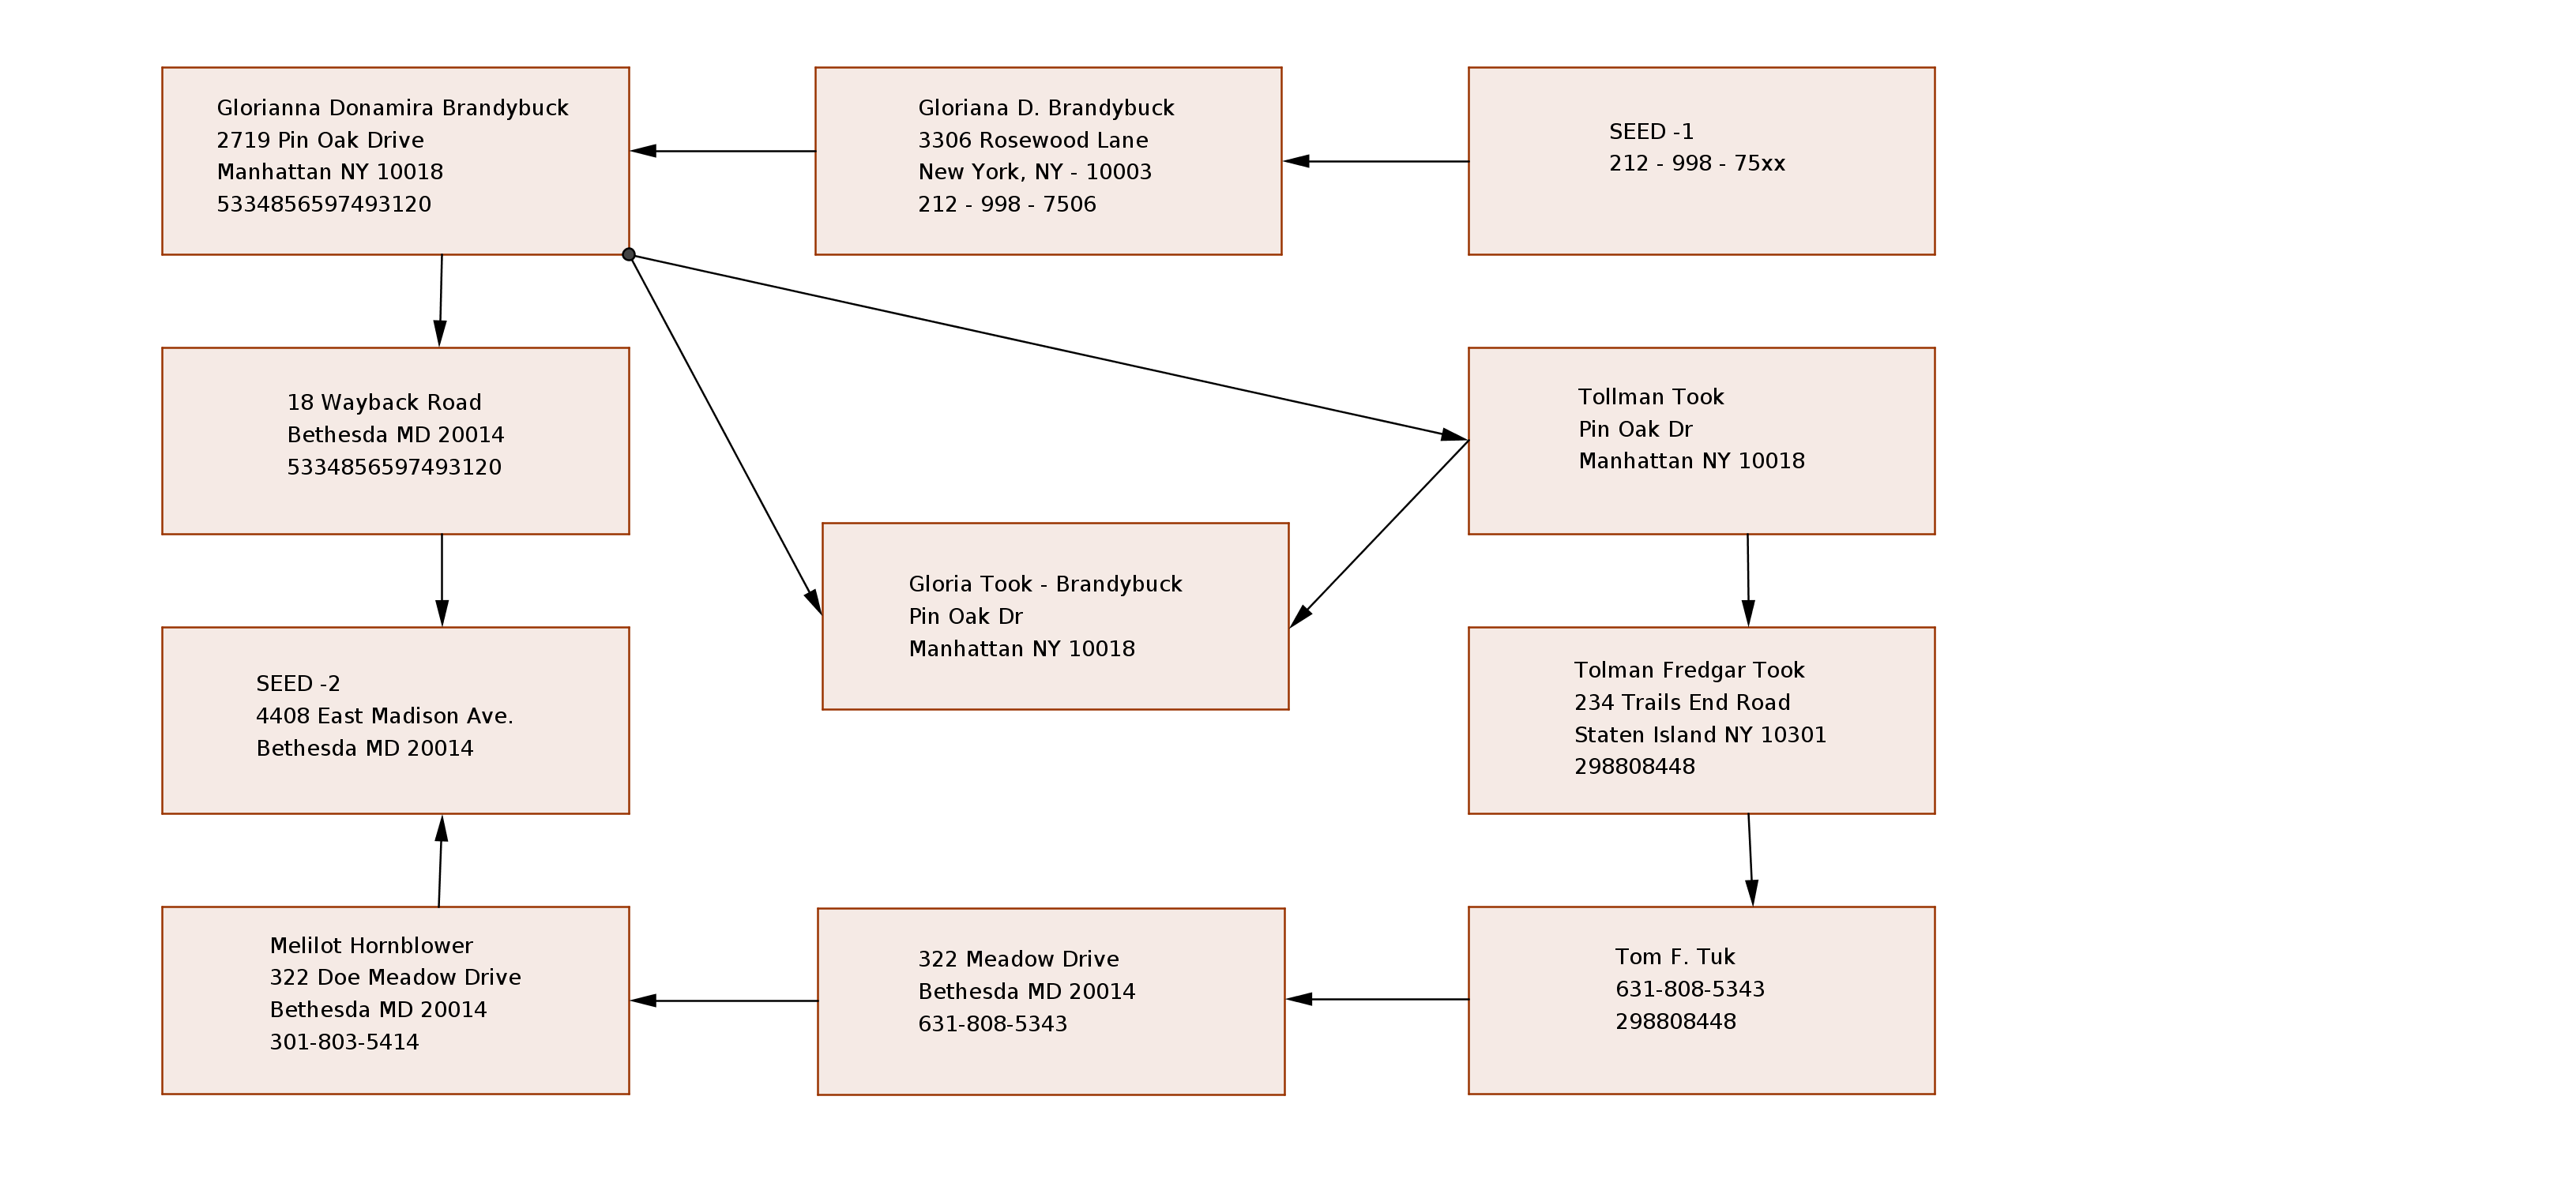
\includegraphics[scale=0.75]{paths.png}
\label{overflow}
\end{figure}

\newpage
\section{Compressive Sensing Techniques}


\subsection{Radon Basis Pursuit}
[Jiang et al] introduced a network data representation framework that allowed for the use of compressive sensing to study the network clique detection problem. They demonstrated that higher-level cliques could be extracted from analysis of a group of people by using radon basis pursuit. Through this approach, the clique detection problem is formulated into a compressive sensing problem.

A network is modeled as a graph $G = (V, E)$, where $V= \{ 1, ..., n \}$ is a set of nodes and $E \subset V \times V$ is the set of edges. A number of important measures are defined as follows: $b$ is a vector of the upper-triangle elements in $B \in  \mathbb{R}^{n \times n}$, the adjacency matrix of a network whose elements indicate the observed frequencies of lower-order subsets; $A$ is an $m \times n$ basis dictionary, with each basis representing a clique; and $x$ is a vector containing the unknown frequencies of higher-order subsets. The reconstruction program used accounted for noise:
\[
(\wp_{1,\delta}) 	min ||x||_1 s.t. ||Ax-b||_{\infty} \leq \delta
\]

However, a number of limitations to this approach include the combinatorial increase in basis size, and the need for a binary weight of edges (i.e. edges are weighed either 0 or 1); thus this approach ultimately was not suitable for our problem. 

%#####

\subsection{Sparse Recovery with Graphs}
Previous work in sparse recovery of graphs has been done in situations in which a weight is associated with each vertex [Wang,Xu, Mallada, Tang]. Using this approach we hoped to obtain communities of nodes similar to the original SEED node. 

Consider the graph $G = (V,E)$, where $V$ is the set of all vertices $x_1 , x_2 , .... , x_n$  and $E$ is the set of edges between any two vertices. Consider only the connected components of $G$. Let $x = \{x_1, x_2, x_3, ... , x_n\}$. Note that $x$ should be sparse since we assume very few nodes are similar to the SEED-1 node. 
Let the support of the vector $x$ be defined to be a vector with its entries being the non-zero indices of $x$, in other words: $\textrm{supp}_x :=\{x_i | x_i \neq  0\}$. Then, $||x||_0 = |\textrm{supp}_x|$. $x$ is defined to be $k$-sparse if $ |\textrm{supp}_x| = k$.

Looking at a subset of nodes  $S \subseteq G$, define $E_S$ as the subset of edges with its vertices in S. Then $G_S = (S,E_S)$ is a induced subgraph of $G$. From here, two assumptions must be made about the measurements of $S$. First, a set of nodes $S$ can be measured iff $G_S$ is a connected subgraph. Secondly, the measurements of $S$ must be additive sums of values at the corresponding nodes. A single specific measurement is obtained by randomly selecting a node in the connected component and performing an additive sum of the tree with depth $h$ from the given node. In relation to the identity challenge, this measurement would represent how similar a particular induced subgraph of $G$ is similar to the SEED node.

Let $y = \{ y_1, y_2, y_3 ... y_m \}$ denote randomly chosen measurements such that $m << n$.  Let $A$ be an $m x n$ measurement matrix such that its $i$th row corresponds to the $i$th measurement.  For a particular entry $A_{ij}$, $A_{ij} = 1$ if  node $j$ is included in the $i$th measurement and $A_{ij} = 0$ otherwise.
Note that we can write the above situation much more compactly as $y = Ax$. This equation is now in the same form used in compressive sensing and sparse recovery.  Compressive sensing theory suggests that the $n$-dimensional vectors can be found from $m$ measurements if the vectors are sparse enough. Therefore $\ell_1$- minimization can be used to recover the sparse vectors using $m$ random measurements.  After the vectors are recovered, the maximal entries in $x$  will denote the nodes most similar to the SEED node. Thus this can be seen as the set of potential disease carriers and a shortest path approach should be able to identify the person.

\subsection{$\ell_1$--minimization}

Given a matrix  A of dimensions M x N with full rank and $y \in \mathbf{R}^M$, look at the equation $min ||x||_1$ s.t. $Ax=b$. An L1 minimization with equality constraintts finds the vector x with the smallest $l_1$ norm. The proceses of finding the smallest x is known as basis pursuit.

\subsection{Implementation}

We implemented majority of our analysis in Python, however, due to lack of good compressed sensing modules for Python, we were forced to use MATLAB for $\ell_1$--minimization process. During our implementation, we discovered a few limitations of the popular L1-Magic library of MATLAB. We were dealing with a massive dataset (350,000 nodes and 68,000 edges); however, the limitations of the library and the hardware we were working on, meant that any data containing with over 18,000 nodes ran out of memory. Hence, we were compelled to make some sacrifices in order to test our approach. 

With the knowledge of correct solution, we realised that we could further prune the search space. We removed all the nodes in the data with just 1 edge incident onto them, the logic being that a node with only one edge cannot lie on to a path that connects the seed nodes. On analysis, we noticed that approximately, 55,000 of the nodes had a degree 1. Removal of these nodes meant drastically altering the structure of the graph. As we further noted, it had a huge impact on the measurement vector $y$ as the depth of the trees is reduced by 1. However, in order to examine the results, we removed these nodes and were left with around 13,500 nodes and their edges. The measurements were consisted of additive sums of the real values of nodes upto a depth of 3. Taking into account the computational cost of this operation, we took 100 measurements. The measurement vector $y$ and the corresponding sensing matrix $A$ are available along with the rest of the code in form of csv files for further examination. However, we ran into more issues with L1-Magic. It couldn't recover the sparse vector $x$ since the matrix ($AA^{T}$) was not a positive definite matrix. We were further forced to sacrifice the accuracy of our data by approximating the matrix to its nearest possible positive definite form. We accomplished this using a library in R. The resultant sparse vector $x$ that we recovered after solving the system contains 99 non-zero entries. The node data corresponding to these non-zero entries is available in form of a csv file. 

The results of our implementation, though hampered by implementation limitations, are fairly encouraging. We can spot a few nodes with the last name 'Took' in our recovered vector. However, we need to further increase the number of measurements upto 1000, to get more insights about the performance of this approach.

\subsection{Further work}

As described above, our experimentation with compressive sensing approach in solving this problem was limited due to implementation issues. Hence, we are keen on further investigating the problem using hardware that can support the heavy computations. We are also keeen on increasing the number of measurements to recover more non-zero values of $x$. In this case, we would need to cluster these non-zero values using k-means to discover community structure of their corresponding nodes. We are also interested in exploring the effect of depth of the measurements and number of measurements on the accuracy of the community structure. 


\section{Conclusion}
Our experiments suggest that path discovery can be a viable method for determning the relationship between two pieces of information. Based upon the nature of data, the iterations of shortest path algorithms can be very sucessful, faster than the compressed sensing approach. Regression can be also highly useful in our specific problem to infer the information necessary to create new edges between two nodes; however is computationally too expensive. Our experiments using compressive sensing suggest that sparse recovery can give an effective subset of nodes to investigate. However further work needs to be done, in making sparse recovery return more useful information as well as more efficient.


\subsubsection*{References}
\small{
%% the NIPS site states that any citation style is fine, as long as you number the references - I used IEEE format but this can be changed if needed (JY)
%% http://dal.ca.libguides.com/content.php?pid=860&sid=11818#ieexapa

%%% PLEASE NUMBER THESE

% Candes/Romberg/Tao's original paper
% http://statweb.stanford.edu/~candes/papers/ExactRecovery.pdf
% http://statweb.stanford.edu/~candes/papers/OptimalRecovery.pdf

[A0] E. Cand\'{e}s, J. Romberg, and T. Tao, "Robust uncertainty principles: Exact signal reconstruction from highly incomplete frequency information," {\it IEE Trans. Inform. Theory}, vol. 52, no.2, pp.489-509, Feb. 2006.

[A1] E. Cand\'{e}s and T. Tao, "Near optimal signal recovery from random projections: Universal encoding strategies?" {\it IEEE Trans. Inform. Theory}, vol. 52, no. 12, pp. 5406-5425, Dec. 2006.

[A2] D. L. Donoho, "Compressed sensing," {\it IEEE Trans. Inform. Theory}, vol. 52, no. 4, pp. 1289-1306, Apr. 2006.

% http://dsp.rice.edu/sites/dsp.rice.edu/files/cs/CSintro.pdf
[A3] E. Cand\'{e}s and M. B. Wakin, "An introduction to compressive sampling," {\it IEEE Signal Process. Mag.}, vol. 25, no. 2, pp. 21-30, Mar. 2008.


% 3 papers on compressive sensing for networked data
% microsoft paper
% correlated compressive sensing for networked data
% http://research.microsoft.com/en-us/um/people/moscitho/Publications/UAI_2014.pdf

[B] T. Shi, D. Tang, L. Xu, and T. Moscibroda, "Correlated compressive sensing for networked data," in {\it The 30th Conference on Uncertainty in Artificial Intelligence (UAI)}, 2014, pp. 722-731.

%http://ieeexplore.ieee.org/xpl/articleDetails.jsp?reload=true&arnumber=6542417
%http://web.engr.illinois.edu/~eslamim2/publications/Siyari-SocialInf12.pdf
[C] P. Siyari, H.R. Rabiee, M. Salehi, and M. Mehdiabadi, "Network reconstruction under compressive sensing," in {\it 2012 International Conference on Social Informatics}, 2012, pp. 19-25.

% http://www.ece.umn.edu/~luo../jdhaupt/publications/spmag07_cs_networked_data.pdf
[D] J. Haupt, W. U. Bajwa, M. Rabbat, and R. Nowak, "Compressed sensing for networked data," {\it IEEE Signal Process. Mag.}, vol. 25, no. 2, pp. 92-101, Mar. 2008.

% MRI http://www.ncbi.nlm.nih.gov/pubmed/17969013
[E] M. Lustig, D. Donoho, and J. M. Pauly, "Sparse MRI: The application of compressed sensing for rapid MR imaging," {\it Magn. Reson. Med.}, vol. 58, no. 6, 1182-1195, Oct. 2007.

%  Genetic screening http://pluto.huji.ac.il/~orzu/publications/Erlich_et_al_allerton_2009.pdf
[F] Y. Erlich, N. Shental, A. Amir, and O. Zuk, "Compressed sensing approach for high throughput carrier screen," in {\it 47th Annual Allerton Conference on Communication, Control}, 2009, pp. 539-544.

% Grouping epidemiology, http://arxiv.org/pdf/1009.3186.pdf
[G] M. Cheraghchi, A. Hormati, A. Karbasi, and M. Vetterli, "Group testing with probabilistic tests: Theory, design and application," {\it IEEE Trans. Inform. Theory,} vol. 57,  no. 10, pp. 7057-7067, Jul. 2011.

%%%% Compressive sensing algorithms

%http://jmlr.org/proceedings/papers/v22/jiang12/jiang12.pdf
[X] X. Y. Jiang, Y. Yao, H. Liu, and L. Guibas, "Detecting network cliques with radon basis pursuit," in {\it Proceedings of the 15th International Conference on Artificial Intelligence and Statistics (AISTATS)}, 2012, pp. 565-573.

%http://people.ece.cornell.edu/atang/pub/12/Infocom12.pdf
[Z] M. Wang, W. Xu, E. Mallada, and A. Tang, "Sparse recovery with graph constraints: Fundamental limits and measurement construction," in {\it 2012 Proceedings IEEE INFOCOM}, 2012, pp. 1871-1879.


\end{document}